\apendice{Especificación de Requisitos}

\section{Introducción}
En este anexo se van a especificar cuales son los requisitos que debe cumplir la aplicación una vez finalizada.

La especificación de requisitos sirve tanto para definir el contrato que se estable entre el cliente con el desarrollador, como para la definición formal del análisis de la aplicación.

\section{Objetivos generales}
Los objetivos del proyecto son crear un entorno donde poder desarrollar, estudiar y probar un vehículo autónomo de forma próxima a como se comportaría en la realidad.

En la aplicación final se podrán probar diferentes configuraciones y algoritmos para poder ver y analizar como afectan al comportamiento del vehículo y cuál de ellas es la más apropiada.

\section{Catálogo de requisitos}

\subsection{Requisitos funcionales}

\begin{itemize}
\tightlist

\item \textbf{RF-1 Simulación del vehículo:} la aplicación tiene que ser capaz de simular el comportamiento de un vehículo de forma realista.
  
\item \textbf{RF-2 Configurar escenario:} el usuario debe poder configurar el mapa, colocando obstáculos, modificando la posición del coche y de la meta.
  
\item \textbf{RF-3 Elección de los algoritmos:} el usuario debe poder elegir que algoritmo usar y probar con los parámetros necesarios.

\item \textbf{RF-4 Visualización de los algoritmos:} la aplicación debe mostrar el procedimiento seguido por los algoritmos.
  
  \begin{itemize}
  \tightlist
  \item \textbf{RF-4.1 Visualización del calculo de la ruta:} la aplicación mostrará como se desarrolla la búsqueda de la ruta de forma gráfica.
  
  \item \textbf{RF-4.2 Visualización de la ruta:} la aplicación mostrará la ruta obtenida.
  
  \item \textbf{RF-4.3 Visualización de los mapas:} la aplicación mostrará los mapas usados para la búsqueda de la ruta.
  \end{itemize}

\item \textbf{RF-5 Preparación de la ruta:} la aplicación será capaz de procesar la ruta obtenida para adecuarla a la realidad.

  \begin{itemize}
  \tightlist
  \item \textbf{RF-5.1 Obtener ruta sin suavizar:} el usuario podrá elegir la ruta sin suavizar tal como la obtenga el algoritmo seleccionado.
  
  \item \textbf{RF-5.2 Obtener ruta suavizada:} el usuario podrá elegir la ruta suavizada seleccionando el modo.

  \end{itemize}

\item \textbf{RF-6 Seguimiento de la ruta:} la aplicación será capaz de mover el vehículo siguiendo las rutas obtenidas.

  \begin{itemize}
  \tightlist
  \item \textbf{RF-6.1 Realizar seguimiento manual:} el usuario podrá elegir seguir la ruta con el vehículo de forma manual.
  
  \item \textbf{RF-6.2 Realizar desplazamiento automático:} el usuario podrá elegir que el vehículo se desplace por la ruta sin tener en cuenta las limitaciones físicas.
  
  \item \textbf{RF-6.3 Realizar seguimiento autónomo:} el usuario podrá elegir que el vehículo siga la ruta de forma autónoma de una forma realista.

  \end{itemize}
  
\end{itemize}

\subsection{Requisitos no funcionales}

\begin{itemize}
\tightlist

\item \textbf{RNF-1 La aplicación debe ser amigable:} debe ser fácil de usar y las representaciones de los algoritmos fáciles de entender.
  
\item \textbf{RNF-2 La aplicación debe ser escalable:} debe poder añadirse algoritmos y nuevas funcionalidades en el futuro de forma sencilla.

\end{itemize}

\newpage
\section{Especificación de requisitos}
En esta sección se especificarán los casos de uso de la aplicación.

En la figura \ref{fig:diagramadecasodeuso} se muestra el diagrama con los casos de uso de la aplicación.

\begin{figure}[htpb]
    \centering
    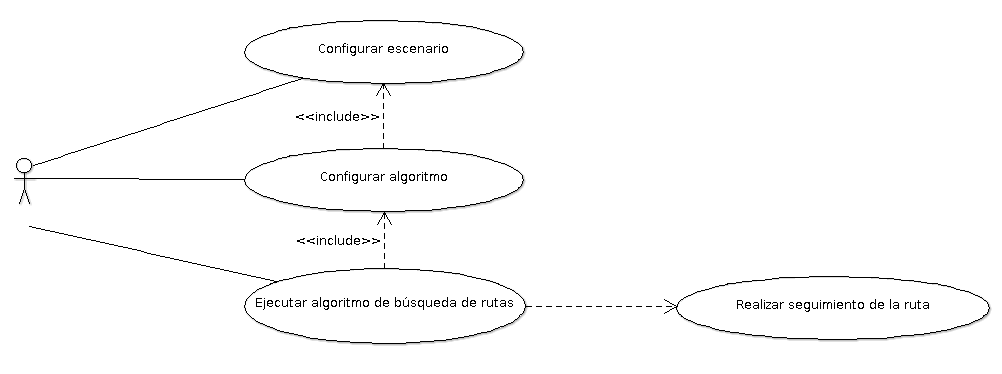
\includegraphics[width=\textwidth,height=10cm,keepaspectratio=true]{b_diagramadecasodeuso}
    \caption[Diagrama de casos de uso]{Diagrama de casos de uso.}
    \label{fig:diagramadecasodeuso}
\end{figure}

%Caso de uso 1
\begin{longtable}[H]{@{}ll@{}}
\toprule
\begin{minipage}[b]{0.23\columnwidth}\raggedright\strut
\textbf{CU-01}\strut
\end{minipage} & \begin{minipage}[b]{0.71\columnwidth}\raggedright\strut
\textbf{Configurar escenario}\strut
\end{minipage}\tabularnewline
\midrule
\endhead

%Version
\begin{minipage}[t]{0.23\columnwidth}\raggedright\strut
\textbf{Versión}\strut
\end{minipage} & \begin{minipage}[t]{0.71\columnwidth}\raggedright\strut
1.0\strut
\end{minipage}\tabularnewline

%requisitos
\begin{minipage}[t]{0.23\columnwidth}\raggedright\strut
\textbf{Requisitos}\strut
\end{minipage} & \begin{minipage}[t]{0.71\columnwidth}\raggedright\strut
RF-2\strut
\end{minipage}\tabularnewline

%descripcion
\begin{minipage}[t]{0.23\columnwidth}\raggedright\strut
\textbf{Descripción}\strut
\end{minipage} & \begin{minipage}[t]{0.71\columnwidth}\raggedright\strut
El usuario puede modificar el escenario por donde se moverá el vehículo.\strut
\end{minipage}\tabularnewline

%precondicion
\begin{minipage}[t]{0.23\columnwidth}\raggedright\strut
\textbf{Precondición}\strut
\end{minipage} & \begin{minipage}[t]{0.71\columnwidth}\raggedright\strut\strut
\end{minipage}\tabularnewline

%acciones
\begin{minipage}[t]{0.23\columnwidth}\raggedright\strut
\textbf{Acciones}\strut
\end{minipage} & \begin{minipage}[t]{0.71\columnwidth}\raggedright\strut
\begin{enumerate}
\def\labelenumi{\arabic{enumi}.}
\tightlist
\item
  El usuario entra en la aplicación.
\item
  Se muestran los obstáculos por defecto, el vehículo y la meta.
\item
  Por cada elemento se muestra los parámetros modificables.
\item
  El usuario modifica los parámetros de los elementos actuales o añade/elimina obstáculos.
\end{enumerate}\strut
\end{minipage}\tabularnewline

%postcondicion
\begin{minipage}[t]{0.23\columnwidth}\raggedright\strut
\textbf{Postcondición}\strut
\end{minipage} & \begin{minipage}[t]{0.71\columnwidth}\raggedright\strut
Debe haber al menos la meta y el vehículo.\strut
\end{minipage}\tabularnewline

%importancia
\begin{minipage}[t]{0.23\columnwidth}\raggedright\strut
\textbf{Importancia}\strut
\end{minipage} & \begin{minipage}[t]{0.71\columnwidth}\raggedright\strut
Alta\strut
\end{minipage}\tabularnewline

%etiqueta
\bottomrule
\caption{CU-01: Configurar escenario.}
\end{longtable}


%Caso de uso 2
\begin{longtable}[H]{@{}ll@{}}
\toprule
\begin{minipage}[b]{0.23\columnwidth}\raggedright\strut
\textbf{CU-02}\strut
\end{minipage} & \begin{minipage}[b]{0.71\columnwidth}\raggedright\strut
\textbf{Configurar algoritmo}\strut
\end{minipage}\tabularnewline
\midrule
\endhead

%Version
\begin{minipage}[t]{0.23\columnwidth}\raggedright\strut
\textbf{Versión}\strut
\end{minipage} & \begin{minipage}[t]{0.71\columnwidth}\raggedright\strut
1.0\strut
\end{minipage}\tabularnewline

%requisitos
\begin{minipage}[t]{0.23\columnwidth}\raggedright\strut
\textbf{Requisitos}\strut
\end{minipage} & \begin{minipage}[t]{0.71\columnwidth}\raggedright\strut
RF-3\strut
\end{minipage}\tabularnewline

%descripcion
\begin{minipage}[t]{0.23\columnwidth}\raggedright\strut
\textbf{Descripción}\strut
\end{minipage} & \begin{minipage}[t]{0.71\columnwidth}\raggedright\strut
El usuario puede elegir el algoritmo a utilizar y modificar sus parámetros.\strut
\end{minipage}\tabularnewline

%precondicion
\begin{minipage}[t]{0.23\columnwidth}\raggedright\strut
\textbf{Precondición}\strut
\end{minipage} & \begin{minipage}[t]{0.71\columnwidth}\raggedright\strut Que exista un escenario válido.\strut
\end{minipage}\tabularnewline

%acciones
\begin{minipage}[t]{0.23\columnwidth}\raggedright\strut
\textbf{Acciones}\strut
\end{minipage} & \begin{minipage}[t]{0.71\columnwidth}\raggedright\strut
\begin{enumerate}
\def\labelenumi{\arabic{enumi}.}
\tightlist
\item
  El usuario entra en la aplicación.
\item
  Se muestran el escenario actual.
\item
  Se muestran los algoritmos disponibles y los parámetros modificables.
\item
  El usuario elige que algoritmo usar, con que opciones y modifica los parámetros disponibles.
\end{enumerate}\strut
\end{minipage}\tabularnewline

%postcondicion
\begin{minipage}[t]{0.23\columnwidth}\raggedright\strut
\textbf{Postcondición}\strut
\end{minipage} & \begin{minipage}[t]{0.71\columnwidth}\raggedright\strut
\strut
\end{minipage}\tabularnewline

%importancia
\begin{minipage}[t]{0.23\columnwidth}\raggedright\strut
\textbf{Importancia}\strut
\end{minipage} & \begin{minipage}[t]{0.71\columnwidth}\raggedright\strut
Alta\strut
\end{minipage}\tabularnewline

%etiqueta
\bottomrule
\caption{CU-02: Configurar algoritmo.}
\end{longtable}


%Caso de uso 3
\begin{longtable}[H]{@{}ll@{}}
\toprule
\begin{minipage}[b]{0.23\columnwidth}\raggedright\strut
\textbf{CU-03}\strut
\end{minipage} & \begin{minipage}[b]{0.71\columnwidth}\raggedright\strut
\textbf{Ejecutar algoritmo de búsqueda de rutas}\strut
\end{minipage}\tabularnewline
\midrule
\endhead

%Version
\begin{minipage}[t]{0.23\columnwidth}\raggedright\strut
\textbf{Versión}\strut
\end{minipage} & \begin{minipage}[t]{0.71\columnwidth}\raggedright\strut
1.0\strut
\end{minipage}\tabularnewline

%requisitos
\begin{minipage}[t]{0.23\columnwidth}\raggedright\strut
\textbf{Requisitos}\strut
\end{minipage} & \begin{minipage}[t]{0.71\columnwidth}\raggedright\strut
RF-3, RF-4, RF-4.1, RF-4.2, RF-4.3, RF-5, RF-5.1, RF-5.2\strut
\end{minipage}\tabularnewline

%descripcion
\begin{minipage}[t]{0.23\columnwidth}\raggedright\strut
\textbf{Descripción}\strut
\end{minipage} & \begin{minipage}[t]{0.71\columnwidth}\raggedright\strut
Se ejecutará el algoritmo seleccionado por el usuario con los parámetros correspondiente y se realizará la visualización del mismo.\strut
\end{minipage}\tabularnewline

%precondicion
\begin{minipage}[t]{0.23\columnwidth}\raggedright\strut
\textbf{Precondición}\strut
\end{minipage} & \begin{minipage}[t]{0.71\columnwidth}\raggedright\strut Que exista un escenario válido.\strut
\end{minipage}\tabularnewline

%acciones
\begin{minipage}[t]{0.23\columnwidth}\raggedright\strut
\textbf{Acciones}\strut
\end{minipage} & \begin{minipage}[t]{0.71\columnwidth}\raggedright\strut
\begin{enumerate}
\def\labelenumi{\arabic{enumi}.}
\tightlist
\item
  El usuario entra en la aplicación.
\item
  Se muestra el escenario actual.
\item
  Se muestran los algoritmos y los parámetros actuales.
\item
  El usuario pulsa el botón de ejecución.
\item
  Si están disponibles y seleccionados, se muestran los mapas correspondientes.
\item
  Si está seleccionado, se muestra el desarrollo del algoritmo.
\item
  Si está seleccionado, se realiza la preparación de la ruta con el método elegido.
\item
  Cuando finalice la búsqueda del algoritmo, se muestra la ruta obtenida.
\end{enumerate}\strut
\end{minipage}\tabularnewline

%postcondicion
\begin{minipage}[t]{0.23\columnwidth}\raggedright\strut
\textbf{Postcondición}\strut
\end{minipage} & \begin{minipage}[t]{0.71\columnwidth}\raggedright\strut
\strut
\end{minipage}\tabularnewline

%importancia
\begin{minipage}[t]{0.23\columnwidth}\raggedright\strut
\textbf{Importancia}\strut
\end{minipage} & \begin{minipage}[t]{0.71\columnwidth}\raggedright\strut
Alta\strut
\end{minipage}\tabularnewline

%etiqueta
\bottomrule
\caption{CU-03: Ejecutar algoritmo de búsqueda de rutas.}
\end{longtable}


%Caso de uso 4
\begin{longtable}[H]{@{}ll@{}}
\toprule
\begin{minipage}[b]{0.23\columnwidth}\raggedright\strut
\textbf{CU-04}\strut
\end{minipage} & \begin{minipage}[b]{0.71\columnwidth}\raggedright\strut
\textbf{Realizar seguimiento de la ruta}\strut
\end{minipage}\tabularnewline
\midrule
\endhead

%Version
\begin{minipage}[t]{0.23\columnwidth}\raggedright\strut
\textbf{Versión}\strut
\end{minipage} & \begin{minipage}[t]{0.71\columnwidth}\raggedright\strut
1.0\strut
\end{minipage}\tabularnewline

%requisitos
\begin{minipage}[t]{0.23\columnwidth}\raggedright\strut
\textbf{Requisitos}\strut
\end{minipage} & \begin{minipage}[t]{0.71\columnwidth}\raggedright\strut
RF-1, RF-6, RF-6.1, RF-6.2, RF-6.3\strut
\end{minipage}\tabularnewline

%descripcion
\begin{minipage}[t]{0.23\columnwidth}\raggedright\strut
\textbf{Descripción}\strut
\end{minipage} & \begin{minipage}[t]{0.71\columnwidth}\raggedright\strut
El vehículo seguirá la ruta obtenida desde la posición inicial del vehículo hasta la meta.\strut
\end{minipage}\tabularnewline

%precondicion
\begin{minipage}[t]{0.23\columnwidth}\raggedright\strut
\textbf{Precondición}\strut
\end{minipage} & \begin{minipage}[t]{0.71\columnwidth}\raggedright\strut Que se haya encontrado una ruta desde la posición inicial del vehículo hasta la meta.\strut
\end{minipage}\tabularnewline

%acciones
\begin{minipage}[t]{0.23\columnwidth}\raggedright\strut
\textbf{Acciones}\strut
\end{minipage} & \begin{minipage}[t]{0.71\columnwidth}\raggedright\strut
\begin{enumerate}
\def\labelenumi{\arabic{enumi}.}
\tightlist
\item
  El usuario entra en la aplicación.
\item
  Se muestra el escenario actual.
\item
  Se muestran los algoritmos y los parámetros actuales.
\item
  El usuario pulsa el botón de ejecución.
\item
  Si el usuario ha elegido el control manual, el vehículo se desplazará con las teclas del teclado.
\item
  Si el usuario ha elegido el desplazamiento automático, el vehículo se trasladará a través de la ruta ignorando las físicas.
\item
  Si el usuario ha elegido el seguimiento autónomo, el vehículo se moverá siguiendo la ruta por si mismo, teniendo en cuenta las físicas para un comportamiento realista.
\end{enumerate}\strut
\end{minipage}\tabularnewline

%postcondicion
\begin{minipage}[t]{0.23\columnwidth}\raggedright\strut
\textbf{Postcondición}\strut
\end{minipage} & \begin{minipage}[t]{0.71\columnwidth}\raggedright\strut
\strut
\end{minipage}\tabularnewline

%importancia
\begin{minipage}[t]{0.23\columnwidth}\raggedright\strut
\textbf{Importancia}\strut
\end{minipage} & \begin{minipage}[t]{0.71\columnwidth}\raggedright\strut
Alta\strut
\end{minipage}\tabularnewline

%etiqueta
\bottomrule
\caption{CU-04: Realizar seguimiento de la ruta.}
\end{longtable}
